\documentclass[12pt]{article}
\usepackage[utf8]{inputenc}

\usepackage{tabularx}
\usepackage{multirow}
\usepackage{graphicx}


\usepackage[legalpaper, margin=1in]{geometry} % landscape

\newcommand*{\addheight}[2][.5ex]{%
  \raisebox{0pt}[\dimexpr\height+(#1)\relax]{#2}%
}

\begin{titlepage} 
2017-1 Term Project Report
\vspace{5cm}

{\huge \centering Title:  \\ Facial emotion recognition with \\ latent topics modeling on local features}

\vspace{5cm}
{
\large
\centering
Date: June 2019

Department: Electronics and Computer Engineering

Name: Vo Thanh Hung

}
\end{titlepage}

\begin{document}


\newpage
% \maketitle

% \begin{table}[]
% % \begin{tabularx}{\textwidth}{X}
% \begin{tabular}{|l|l|l|l|l|l|}
% \hline
% \begin{tabular}[c]{@{}l@{}}Project\\ Title\end{tabular} & \multicolumn{3}{c|}{\textbf{\begin{tabular}[c]{@{}l@{}}Facial emotion recognition\\ with latent topics modeling\\ on local features\end{tabular}}} & Date & 2019.05.27 \\ \hline
% Name & \hspace{.5cm} Vo Thanh Hung \hspace{.5cm} & Student ID & \hspace{0.5cm} 198554 \hspace{0.5cm} & Evaluation &  \\ \hline
% \end{tabular}
% \end{table}
% % \end{tabularx}


\section{Introduction}
% In this section
% - Why do you do this project?
% - Why is this project important?
% Etc., describe the background, necessity and importance of the project.

In this study, I am going to discover re-presentation of image features and apply to facial emotion recognition (FER) problem.
There are many feature extraction method including Scale Invariant Feature Transform \cite{Lowe2004} (SIFT), Speeded Up Robust Features \cite{Bay06} (SURF), KAZE features \cite{alcantarilla2012kaze}, etc.
In this project, SIFT, SURF and KAZE are used.
Each of above method will generate a set of vector from given image.
To use extracted features to most of recognition problem, we have to re-presentation them.
Bag-of-Features \cite{nowak2006sampling} was wide used for this step which the idea transform from Bag-of-Words in natural language processing (NLP).
In this study, I address not only one kind of feature, but also multi-features kind, meaning from some difference feature extraction method.
So, I hope that the result can be improve and general compared to single method.

I am going to apply for FER problem and on some special popular dataset.
The problem is expected that combine many type of local features can present and easy understand emotion in image.
% There are another assumption, that facial features are not change too much and prevent with many [TO-DO pose]...

After that, some popular traditional machine learning methods are used to facial emotion recognition including Support Vector Machine \cite{suykens1999least} (SVM), Random Forest \cite{liaw2002classification}.

\section{Related Research and Key Technology}
% - Describe some of the key skills required to carry out the project.
% - Summarize the necessary related knowledge about artificial intelligence technology used for the project..
Many related technologies are show as below.

% [TO-DO feature]

Feature extraction:
\begin{itemize}
    \item Scale Invariant Feature Transform \cite{Lowe2004} (SIFT)
    \item Speeded Up Robust Features \cite{Bay06} (SURF)
    \item KAZE features \cite{alcantarilla2012kaze}
    % \item \cite{Pang2012} 
    % \item \cite{Sun:2016:EMV:2988257.2988270}
\end{itemize}

% [TO-DO feature normalization]

% [TO-DO LDA, HDP]
Topics modeling:
\begin{itemize}
    \item Latent Dirichlet Allocation \cite{blei2003latent, Blei2003} (LDA)
    \item Hierarchical Dirichlet Process \cite{teh2005sharing} (HDP)
\end{itemize}

% [TO-DO machine learning]
Machine learning classifier:
\begin{itemize}
    \item Naive Bayes (NB)
    \item Support Vector Machine \cite{suykens1999least} (SVM)
    \item Random Forest \cite{liaw2002classification} (RF)
\end{itemize}

% [TO-DO? transfer model]

\section{Project Contents and Algorithm} \label{sec:project-contents}
% In this section, you will write something about the actual
% - Structure of system
% - Basic algorithm
% - Specific implementation details, etc.


% [TO-DO add system architect]
Figure \ref{fig:system-architect} show overall system architect.
The input image goes through feature extractor block to get all features.
These block including SIFT, SURF and KAZE.
Then Bag-of-Features does clustering and make fixed vocabulary.
From here, there are two branches to implement two difference approaches.
First approach is to directly use Bag-of-Features and classifier.
The other approach is to modeling features use HDP and then represent image before goes through classifier block as previous.
Two approaches work independence to compare.
\begin{figure}[h!]
    \centering
    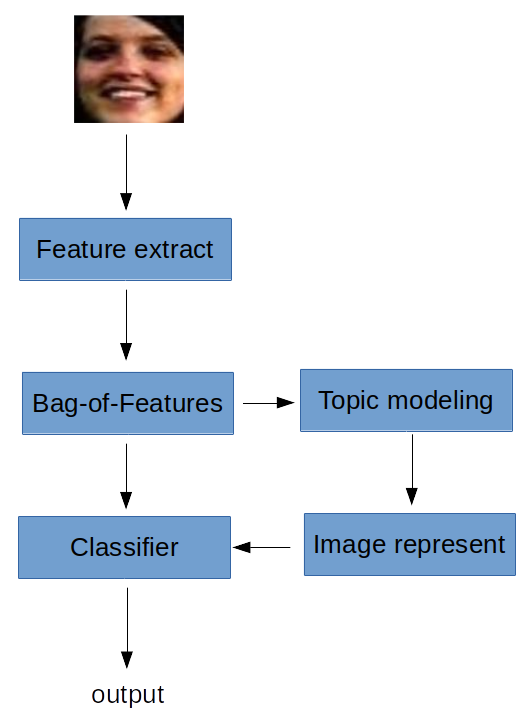
\includegraphics[width=0.45\textwidth]{system-arch-cropped.png}
    \caption{Facial emotion recognition system architect} \label{fig:system-architect}
\end{figure}

Below subsections show description for each block.

% ----------------------------
% feature extraction
% ----------------------------
\subsection{Features extraction}
This step aims to extract features from images.
The OpenCV toolbox \cite{opencv_library} was used to perform this task.
The input is an image, the output is features.
The feature size of SIFT, SURF and KAZE are 128, 64  and 64, in this order.

After extracted, all features vector are normalize use l2 normalization.

% ----------------------------
% Bag-of-Feature
% ----------------------------
\subsection{Bag-of-Features}
In our case, there are many kind of feature vectors from difference extractor, that mean they have difference size of vector.
The SIFT feature size is 128 while SURF feature size is 64 and similar for KAZE.
Bag-of-Features technique are wide used to represent image features.
From normalized features, the clustering is used to make the number of cluster $K$ based on distance of features.
The K-means clustering algorithm \cite{hartigan1979algorithm} was widely used, and Euclidean distance also used here.
$K$, the number of cluster is number of vocabulary.
All feature belong to one cluster is same \textit{word} which centroid of cluster is represent for them.

Then the image is represent as a vector length $K$, each value in the vector is for one word.
Word order is not considered here.
Term Frequency (TF) for each word is calculated and make vector.
In this case, I am going to use both TF and IDF (Inverse Document Frequency) to make vector and compare result.
Both TF and IDF concepts are come from NLP.


% ----------------------------
% build hdp model for feature
% ----------------------------
\subsection{Features modeling}
This part of study tries to modeling features of image in an another way than Bag-of-Features.
In this project, latent topics modeling are explore, one another techniques from NLP.
The main idea is to discover the related of hidden topics from words, features.

Latent Dirichlet Allocation \cite{blei2003latent, Blei2003} is probabilistic for describing whether a subject are present in each document relative to a given article topic model.
There the number of topics is set and the probabilities of words belongs to each topic and the probabilities of documents belongs to each topic are estimate.
In our case, the words are represent vectors and images are documents.

Hierarchical Dirichlet Process \cite{teh2005sharing} (HDP) is a improvement version of LDA where number of topic need not given, they will be estimate too.

There are some use case and modified version of LDA and HDP were studied by Hu et al. in \cite{Hu2009} and Cao et al. in \cite{Cao2007}.

In this project, I am going to modeling features by latent topic and HDP is used.

% ----------------------------
% classifier
% ----------------------------
% SVM
% Random forest
% NB
% KNN?
\subsection{Classifier}
In this study, we use some popular traditional machine learning to classify including SVM \cite{suykens1999least}, Random forest \cite{liaw2002classification}, Naive Bayes.


\section{Experiment and Result}
\subsection{Dataset}

We use Real-world Affective Faces Database \cite{li2017reliable, li2019reliable} (RAF-DB) for our experiment.
Dataset was separated to training and testing set.
The size of training and testing is 12271 and 3068 images.
There is two different subsets, single-label subset including 7 classes of basic emotions; and two-tab subset, including 12 classes of compound emotions.
In this project, the basic emotion dataset was used.
Figure \ref{fig:raf-db-example} shows some examples images from dataset.
From examples, we can see that some images have clearly emotion when another images is difficult to detect emotion.
This is a real-world image, then face maybe rotate, glasses or some thing may hide face.
Those things make more difficult to detect emotion.

\begin{figure} [h!]
    \centering
\begin{tabular}{|c|c|c|c|c|c|c|}
      \hline
      \small Surprise & Fear & Disgust & Happiness & Sadness & Anger & Neutral \\
      \addheight{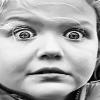
\includegraphics[width=18mm]{imgs/train_00006_aligned-1.jpg}} &
      \addheight{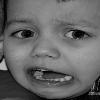
\includegraphics[width=18mm]{imgs/train_00027_aligned-2.jpg}} &
      \addheight{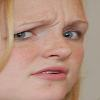
\includegraphics[width=18mm]{imgs/train_00031_aligned-3.jpg}} &
      \addheight{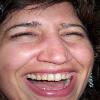
\includegraphics[width=18mm]{imgs/train_00016_aligned-4.jpg}} &
      \addheight{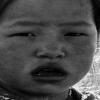
\includegraphics[width=18mm]{imgs/train_00005_aligned-5.jpg}} &
      \addheight{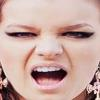
\includegraphics[width=18mm]{imgs/train_00047_aligned-6.jpg}} &
      \addheight{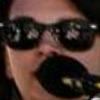
\includegraphics[width=18mm]{imgs/train_09757_aligned-7.jpg}} \\

      \addheight{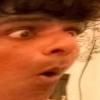
\includegraphics[width=18mm]{imgs/test_0043_aligned-1-2.jpg}} &
      \addheight{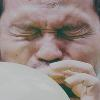
\includegraphics[width=18mm]{imgs/test_0274_aligned-2-2.jpg}} &
      \addheight{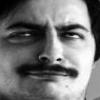
\includegraphics[width=18mm]{imgs/train_09745_aligned-3-2.jpg}} &
      \addheight{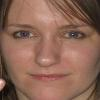
\includegraphics[width=18mm]{imgs/test_0055_aligned-4-2.jpg}} &
      \addheight{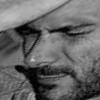
\includegraphics[width=18mm]{imgs/test_0049_aligned-5-2.jpg}} &
      \addheight{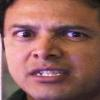
\includegraphics[width=18mm]{imgs/test_0057_aligned-6-2.jpg}} &
      \addheight{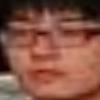
\includegraphics[width=18mm]{imgs/train_09759_aligned-7-2.jpg}} \\
      \hline
\end{tabular}
    \caption{Example image from RAF-DB}
    \label{fig:raf-db-example}
\end{figure}


Table \ref{tbl:raf-db-count} show the number image for each classes.
We can see that the dataset is high unbalanced.
In both training set and testing set, the number of \textit{Happiness} class are nearly three times of average with 4772 and 1185, respective.
The second high number of image is \textit{Neutral} with 2524 and 680 images on training and testing, respective.
The lowest number of image is \textit{Fear}, there are only 281 on training and 74 on testing.
Unbalanced is normalize in the facial emotion dataset because in natural, we can easy found the \textit{happiness} and \textit{neutral} emotion than \textit{fear} or \textit{anger}.

\begin{table}[h!]
\centering
\caption{Number image in each class for training and testing in RAF-DB} \label{tbl:raf-db-count}
\begin{tabular}{|l|c|c|}
\hline
\textbf{Class} & \textbf{Training} & \textbf{Testing} \\ \hline
Surprise & 1290 & 329 \\ \hline
Fear & 281 & 74 \\ \hline
Disgust & 717 & 160 \\ \hline
Happiness & 4772 & 1185 \\ \hline
Sadness & 1982 & 478 \\ \hline
Anger & 705 & 162 \\ \hline
Neutral & 2524 & 680 \\ \hline \hline
\textbf{Average} & \textbf{1753} & \textbf{438} \\ \hline
\textbf{Total} & \textbf{12271} & \textbf{3068} \\ \hline
\end{tabular}
\end{table}

We all know that unbalanced in dataset will have large affect on model.
In this study, we report the results on both original (unbalanced) and balanced training data.
The testing data leave as it.

\subsection{Bag-of-Words method}
For Bag-of-Words method, there are two classifier were tested.
Table \ref{tbl:bag-of-words-metric} show accuracy metrics for NB, SVM and RF on unbalance and balanced data.
On both case, SVM gave the best result with 49.0\% on unbalance and 40.64\% on balanced data with large margin compared to the second one is NB about 8-10\%.
RF got the lowest result in balanced data, but better than NB in the unbalance data.
As many research before, SVM still the best algorithm in our dataset.

\begin{table}[h!]
\centering
\caption{Bag-of-Words results, metric accuracy (\%)} \label{tbl:bag-of-words-metric}
\begin{tabular}{|l|l|l|}
\hline
Classifier & Unbalance & Balanced \\ \hline
NB & 41.82 & 30.02 \\ \hline
SVM & 49.0 & 40.64 \\ \hline
RF & 43.80 & 24.37 \\ \hline
\end{tabular}
\end{table}

NB confusion matrix for unbalanced is showed in figure \ref{fig:normal-bow-nb} and figure \ref{fig:upsample-bow-nb} in case of sampling to get balance for classes.
We easily see that on unbalance data, the result get better accuracy, but algorithm predict all images belongs to \textit{Happiness} or \textit{Neutral}.
On balanced data, the confusion matrix is more beautiful, model seems not bias to special classes.
But, in this case, the accuracy is lower than unbalance case, due to the test set also bias too.

\begin{figure} [h!]
    \centering
    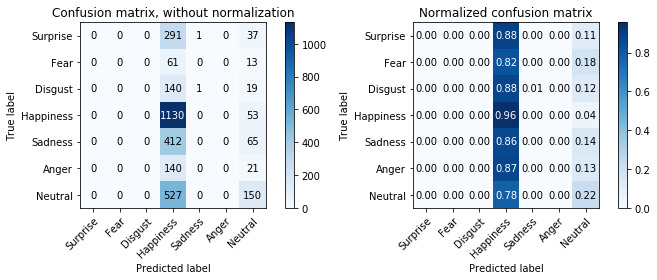
\includegraphics[width=\textwidth]{imgs/n-bow-nb.jpg}
    \caption{Bag-of-Words confusion matrix on unbalance data with NB}
    \label{fig:normal-bow-nb}
\end{figure}

\begin{figure} [h!]
    \centering
    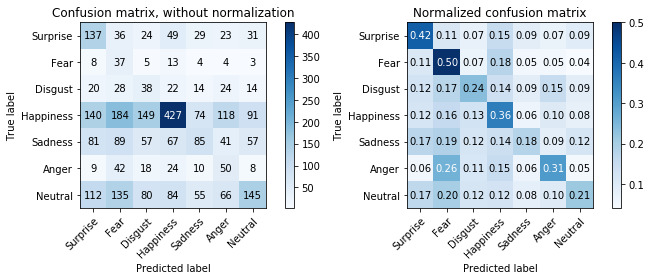
\includegraphics[width=\textwidth]{imgs/upsample-bow-nb.jpg}
    \caption{Bag-of-Words confusion matrix on balanced data with NB}
    \label{fig:upsample-bow-nb}
\end{figure}
       
SVM confusion matrix for unbalance and balanced data when apply SVM algorithm are showed in figure \ref{fig:normal-bow-svm} and figure \ref{fig:upsample-bow-svm}, respective.

As table \ref{tbl:bag-of-words-metric}, the results on SVM better than on NB.
For balanced case, the result does not bias on classes as unbalance data.
Similar NB, accuracy drop because the bias of test set.

\begin{figure} [h!]
    \centering
    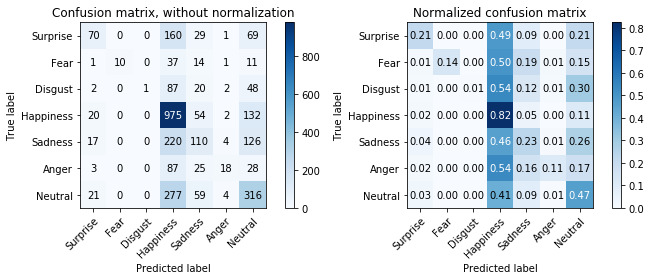
\includegraphics[width=\textwidth]{imgs/n-bow-svm.jpg}
    \caption{Bag-of-Words confusion matrix on unbalance data with SVM}
    \label{fig:normal-bow-svm}
\end{figure}

\begin{figure} [h!]
    \centering
    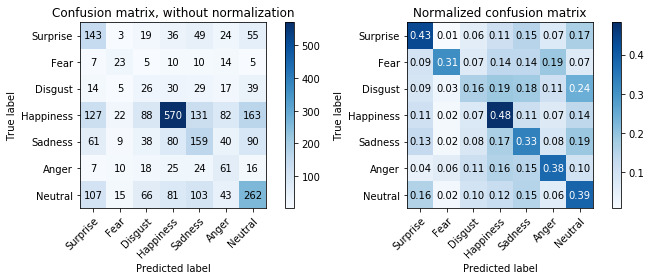
\includegraphics[width=\textwidth]{imgs/upsample-bow-svm.jpg}
    \caption{Bag-of-Words confusion matrix on balanced data with SVM}
    \label{fig:upsample-bow-svm}
\end{figure}

Similar with SVM and NB, the confusion matrix with RF algorithm is showed on figure \ref{fig:bow-rf}.
In this case, the result on balanced data worse, the distribution seems randomly.
It only slighly better than random classifier.

\begin{figure} [h!]
    \centering
    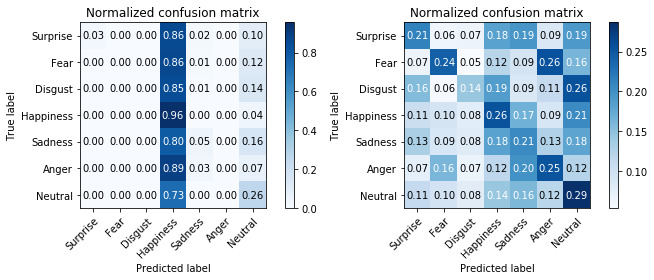
\includegraphics[width=\textwidth]{imgs/bow-rf.jpg}
    \caption{Bag-of-Words confusion matrix with RF}
    \label{fig:bow-rf}
\end{figure}
       
       
\subsection{Topic modeling}       
       
For topic modeling, there are several steps including feature modeling, document represent and finally classification.

Modeling features, I use HDP \cite{teh2005sharing} to modeling with auto reference number of topics.
The bag-of-words of each images then pass to HDP, and after number of iterator, algorithm finish.
The results of the modeling distribution of features and documents.
For RAF-DB dataset and above bag-of-words method, HDP found that there are 150 hidden topics.

In our case, we consider the distribution of each image over hidden topics.
Each image view as one document and then can retrieval the distribution of topics.
An example of distribution of image features based on topics as following: 
[(3, 0.4618), 
  (26, 0.1038),
  (89, 0.0624),
  (128, 0.1699),
  (136, 0.0855),
  (138, 0.0864),
  (148, 0.0241)]
  

%  [(8, 0.7347021583895617),
%   (46, 0.1441341423208861),
%   (79, 0.11680245565832961)],

%  [(1, 0.5838619553442171),
%   (46, 0.05318602792629546),
%   (99, 0.2291244361167196),
%   (101, 0.03952411922636785),
%   (111, 0.08837481488811819)]]

The image has distribution on topics 3, 26, 89, 128, 136, 138 and 148 with probabilities 0.4618, 0.1038, 0.0624, 0.1699, 0.0855, 0.0863, 0.0241 respective.
All other topics have small probabilities (nearly zero or zero) then omit here.
Note that, total probabilities of all topics of each image is one.
We use those spare vector to classify responding image.

The final step is use classifier to classify those vector.

Table \ref{tbl:topic-modeling-metric} show the result on unbalance and balanced data with three algorithm NB, SVM and RF.
The SVM still good enough, although in the balanced there is a small lower than NB.
There are drop accuracy on balance compared to unbalance as Bag-of-Words method.
In this case, it seems that topics modeling do not have good information to classifier.

\begin{table}[h!]
\centering
\caption{Topic modeling results, metric accuracy (\%)} \label{tbl:topic-modeling-metric}
\begin{tabular}{|l|l|l|}
\hline
Classifier & Unbalance & Balanced \\ \hline
NB & 39.89 & 22.90 \\ \hline
SVM & 40.12 & 22.35 \\ \hline
RF & 43.80 & 23.65 \\ \hline
\end{tabular}
\end{table}

\section{Conclusion}
% To be extend:
% \cite{Georgescu2018} for handcrafted features for FER.
% \cite{Feng2010} topic models for image annotation.
In this project, I experiment FER problem that use Bag-of-Words and topic modeling method.
There difference classification methods was experiment and compare results.
The result shows that Bag-of-Words is simple but still better than topic modeling method, that depend on probability modeling.

\textit{Note: Source code is public in GitHub with link: \href{https://github.com/thanhhungqb/AI-theory}}


\bibliographystyle{ieeetr}
\bibliography{library,library-tools,a} 

\end{document}
